\chapter{Analiza wyników}
{

    Jednym z napotkanych problemów podczas implementacji procesu przetwarzania danych i projektu architektury modelu
    był czasochłonny krok oceny wyników. Po każdorazowym uczeniu modelu konieczne było generowanie próbek, 
    konwersja ich postaci numerycznej na pliki midi, manualny odsłuch i subiektywna ocena.

    W celu formalizacji wyników i uzyskania możliwości wygodniejszego sposobu oceny modelu, konieczne było wyznaczenie
    miar opisujących generowane próbki. 

    \section{Miary i ich definicje}
    {
        Na podstawie artykułu 'On the evaluation of generative models in music'\cite{Yang2018OnTE} zdecydowano się zaimplementować następujące miary:
        \begin{itemize}
            \item Rozpiętość tonalna - odległość między najniższym i najwyższym dźwiękiem, w przypadku plików midi ograniczona
            zakresem <0,127>,
            \item Histogram tonalny - rozkład występowania poszczególnych dźwięków z dwunastotonowej skali, niezależnie od oktawy, 
            \item Macierz przejść dźwięków - dwuwymiarowa macierz przedstawiająca częstotliwość występowania par dźwięków następujących
            po sobie. Uwagi wymaga kwestia nanoszenia na macierz informacji o następujących po sobie wielodźwiękach. W celu oddania
            również takich zdarzeń, na macierz nanoszone są pary będące wynikami iloczynu kartezjańskiego między składowymi wielodźwięków.
            \item Rozpiętość rytmiczna - odległość między najkrótszą i najdłuższą wartością rytmiczną występującą w mierzonej próbce. 
            Ponieważ wartości kodu 1 z N są posortowane według długości trwania, może ona być wyrażona poprzez różnicę indeksów 
            między klasami kodu 1 z N. Przyjmuje wartości z zakresu <0, ilość klas rytmicznych>.
            \item Histogram rytmiczny - rozkład występowania poszczególnych klas wartości rytmicznych.
            \item Macierz przejść wartości rytmicznych - opisuje częstość przejść między konkretnymi wartościami rytmicznymi.
        \end{itemize}

        Dodatkowo, opracowano dwie miary mierzące stopień kompresji generowanych ciągów dźwięków i wartości rytmicznych. 
        Uznanie stopnia kompresji jako istotny parametr wynika z intuicji wynikającej z zasady działania dużej części
        algorytmów kompresji, w których powtarzające się ciągi znaków są zastępowane krótszym znacznikiem wskazującym na pierwsze 
        wystąpienie ciągu. 
        Oznacza to, że sekwencje charakteryzujące się większą powtarzalnością mogą zostać skompresowane w większym stopniu.
        Główną zaletą tej miary jest jej zdolność wykrywania powtarzających się ciągów rozsuniętych w czasie, co stanowi uzupełnienie 
        bardziej lokalnej miary, jaką jest macierz przejść.

        W celu możliwości skorzystania z dostępnych algorytmów, sekwencje dźwięków i wartości rytmicznych zostały przekształcone
        na ciągi znaków. W przypadku wektorów opisujących dźwięki zdecydowano się na zapis symboli kolejnych dźwięków. Wartości
        rytmiczne przedstawione były przez indeksy odpowiadających im klas. 

        Do kompresji wykorzystano bibliotekę zlib, korzystającą z algorytmu delfate.
    }

    \section{Pomiar zbioru treningowego}
    {
        Ponieważ wartości miar będą różne dla każdego zbioru danych, w procesie oceny generowanych próbek powinno się je 
        stosować w odniesieniu do wartości wyznaczonych dla całego zbioru danych treningowych.
        
        Na obrazkach \ref{tonal_hist_transition}, \ref{rythm_hist_transition} oraz w tabeli \ref{range_and_compression} 
        przestawione są wartości miar całego zbioru testowego.

        %%% ilustracja tonalnego histogramu i macierzy przejść
        \begin{figure}
            \centering
            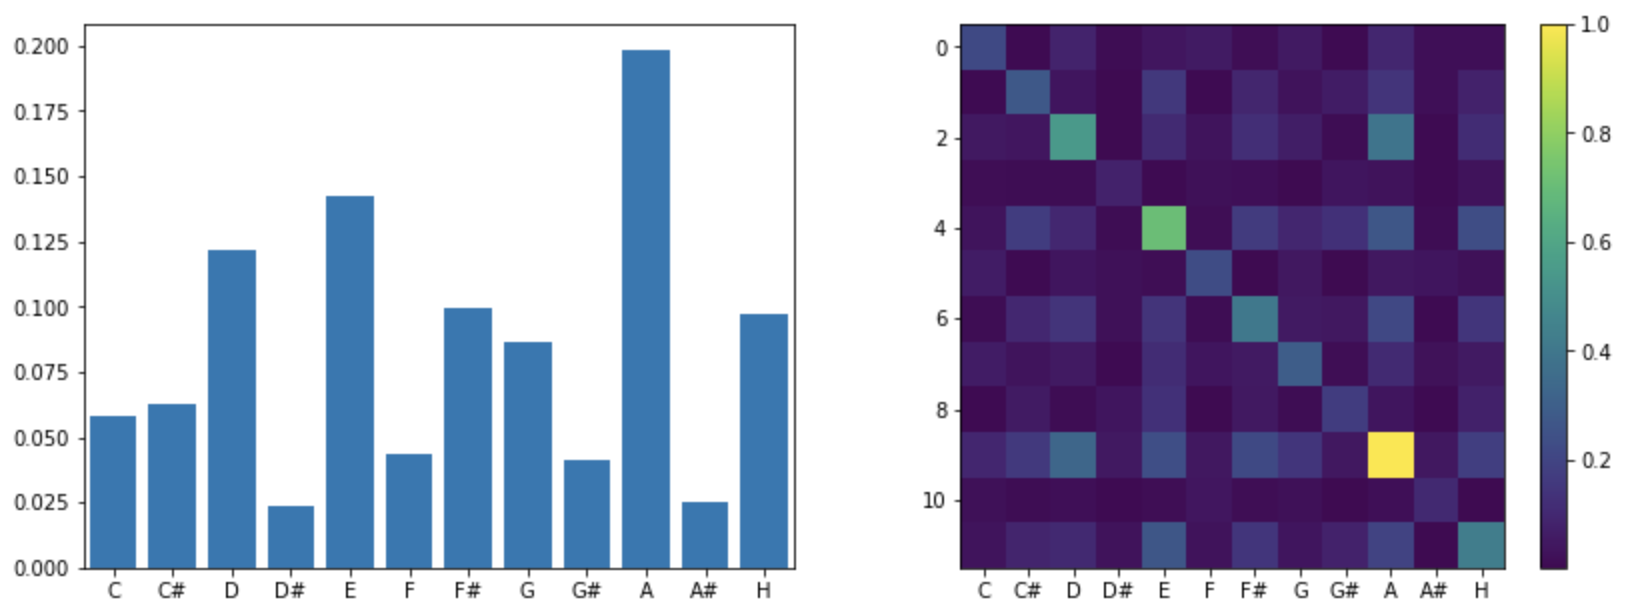
\includegraphics[scale=0.5]{tonal_hist_transition}
            \caption{Histogram występowania poszczególnych dźwięków oraz macierz przejść między nimi}
            \label{tonal_hist_transition}
        \end{figure}

        %%% histogram rytmiczny i macierz przejść
        \begin{figure}
            \centering
            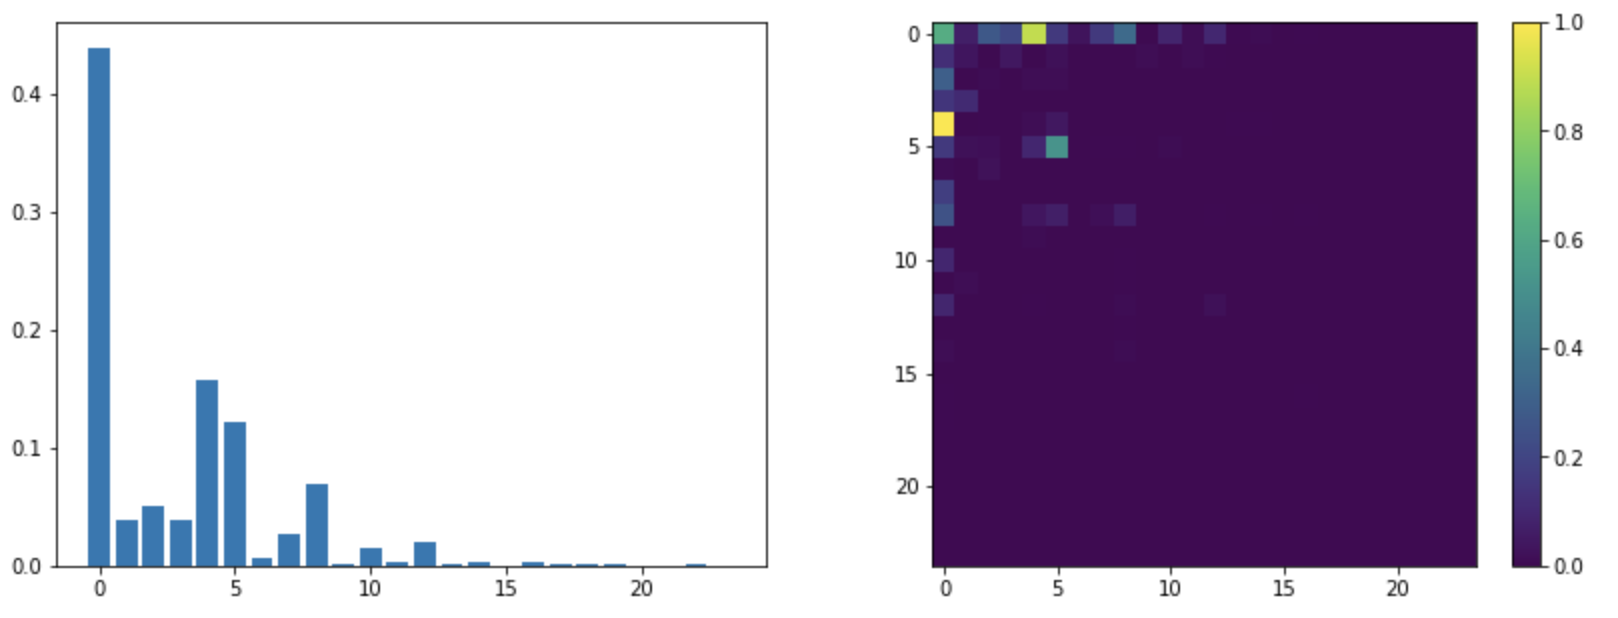
\includegraphics[scale=0.5]{rythm_hist_transition}
            \caption{Histogram występowania poszczególnych długości dźwięków oraz macierz przejść między nimi}
            \label{rythm_hist_transition}
        \end{figure}

        %%% tabelka z zakresami i kompresją
        \begin{table}
            \begin{center}
                \begin{tabular}{ |p{2.5cm}|p{2.5cm}|p{2.5cm}|p{2.5cm}|p{2.5cm}| }
                \hline
                 & Zakres & Współczynnik kompresji \\ 
                \hline
                Wysokość dźwięków & 69 & 6.932 \\  
                \hline
                Długość dźwięków & 23 & 11.364 \\
                \hline
                \end{tabular}
            \end{center}
            \caption{Zakresy i współczynniki kompresji danych} \label{range_and_compression}
        \end{table}

        \pagebreak

        Na postawie wykresów możemy sformułować następujące wnioski:
        \begin{itemize}
            \item najczęściej występującym dźwiękiem w zbiorze jest A, a najrzadszym D\#,
            \item wyższe wartości na przekątnej macierzy przejść dźwięków wskazują, że dźwięk występujący w bieżącym wielodźwięku
            często występuje również w następującym
            \item symetria macierzy przejść dźwięków wskazuje na brak silnego wpływu kierunku odtwarzania utworu na następstwa tonalne
            \item klasy przedstawiające długości trwania dźwięków są silnie niezrównoważone
        \end{itemize}
    }

    \section{Wyniki}
    {
        Kolejnym krokiem było wygenerowanie próbek i opisanie ich za pomocą wymienionych miar. Zestawienie wartości miar i różnic
        w odniesieniu do zbioru treningowego przedstawiają tabele \ref{tonal_measuremnts_table} i \ref{rythm_measuremnts_table}. Wyniki pogrupowano na podstawie użytego ziarna.

        \begin{table}
            \begin{center}
                \begin{tabular}{ |p{2.5cm}|p{2.5cm}|p{2.5cm}|p{2.5cm}|p{2.5cm}| }
                \hline
                Ziarno & Rozpiętość tonalna & Średnia kwadratowa różnicy histogramu tonalnego & Średnia kwadratowa różnicy tonalnej macierzy przejść & Współczynnik kompresji dźwięków \\ 
                \hline
                \hline
                Wartości losowe rozkładu normalnego & 65 & 0.026 & 0.112 & 7.69 \\  
                \hline
                Wektory zerowe & 61 & 0.062 & 0.116 & 9.52 \\
                \hline
                Pojedynczy dźwięk & 67 & 0.025 & 0.111 & 9.83 \\
                \hline
                Sekwencja losowych dźwięków & 69 & 0.023 & 0.120 & 8.84 \\
                \hline
                Harmoniczna sekwencja dźwięków & 69 & 0.021 & 0.106  & 8.78 \\
                \hline
                \end{tabular}
            \end{center}
            \caption{Wyniki miar tonalnych próbek generowanych różnymi ziarnami} \label{tonal_measuremnts_table}
        \end{table}
        
        \begin{table}
            \begin{center}
                \begin{tabular}{ |p{2.5cm}|p{2.5cm}|p{2.5cm}|p{2.5cm}|p{2.5cm}| }
                \hline
                Ziarno & Rozpiętość rytmiczna & Średnia kwadratowa różnicy histogramu rytmicznego & Średnia kwadratowa różnicy rytmicznej macierzy przejść & Współczynnik kompresji długości dźwięków \\ 
                \hline
                \hline
                Wartości losowe rozkładu normalnego & 19 & 0.019 & 0.034 & 7.99 \\  
                \hline
                Wektory zerowe & 16 & 0.035 & 0.059 & 10.4 \\
                \hline
                Pojedynczy dźwięk & 20 & 0.030 & 0.042 & 9.52 \\
                \hline
                Sekwencja losowych dźwięków & 21 & 0.028 & 0.042 & 8.19 \\
                \hline
                Harmoniczna sekwencja dźwięków & 21 & 0.030 & 0.043 & 7.89 \\
                \hline
                \end{tabular}
            \end{center}
            \caption{Wyniki miar rytmicznych próbek generowanych różnymi ziarnami} \label{rythm_measuremnts_table}
        \end{table}

        Występujące różnice między wynikami nie pozwalają na pewne wskazanie najlepszego ziarna, lecz 
        zachęcają do wysunięcia kilku wniosków.

        Wszystkie sekwencje poza inicjowanymi pustymi wektorami dają zbliżone różnice miedzy histogramami i 
        tonalnymi macierzami przejść. 
        Sekwencje zapoczątkowane wartościami losowymi zgodnie z intuicją charakteryzują się niższym współczynnikiem
        kompresji, co może przekładać się na większe zróżnicowanie sekwencji dźwięków.
        Spośród zbadanych ziaren, sekwencje początkowane harmonicznym zestawem dźwięków najwierniej
        odwzorowały rozkłady następujących po sobie dźwięków.
        
        Na obrazku \ref{tonal_hist_transition_1} oraz \ref{rythm_hist_transition_1} zamieszczono uśrednione 
        histogramy i macierze przejść próbek wygenerowanych przy pomocy różnych ziaren.

        %%% wykresiki
        %%% ilustracja tonalnego histogramu i macierzy przejść
        \begin{figure}
            \centering
            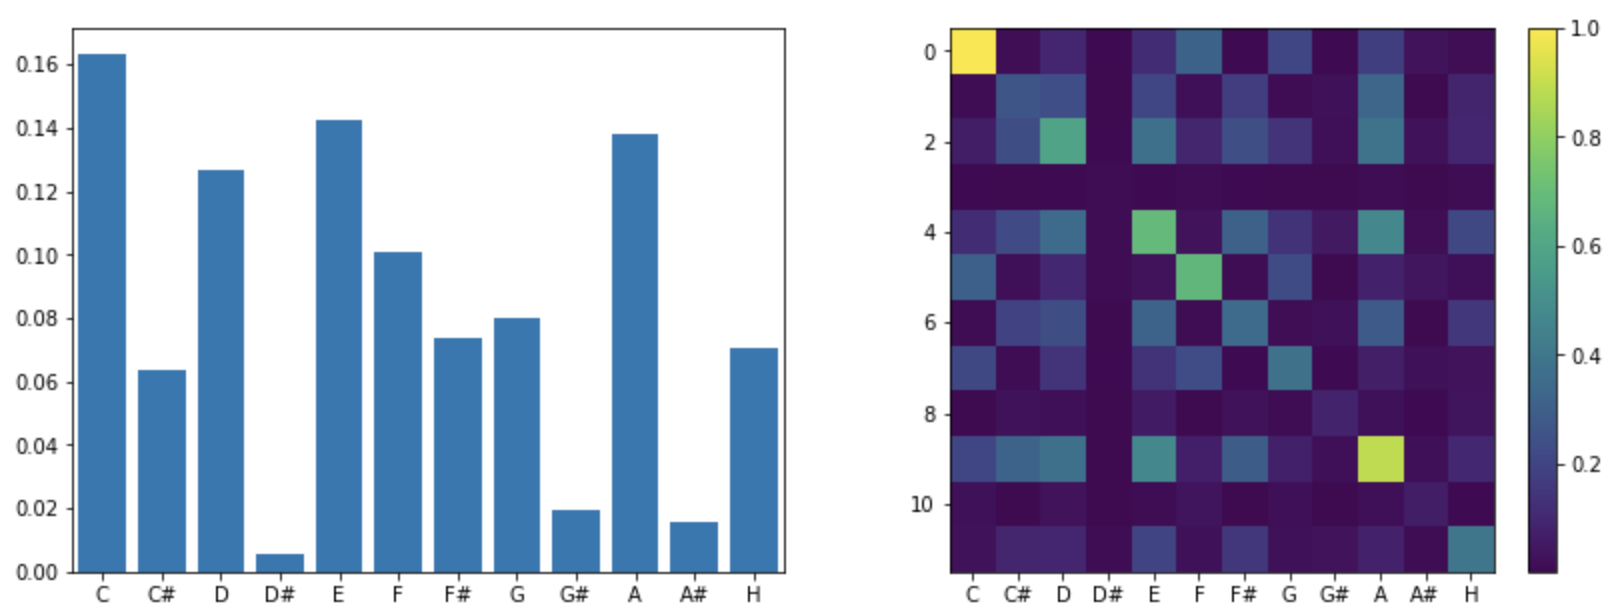
\includegraphics[scale=0.5]{tonal_hist_transition_1}
            \caption{Histogram występowania poszczególnych dźwięków oraz macierz przejść między nimi}
            \label{tonal_hist_transition_1}
        \end{figure}

        %%% histogram rytmiczny i macierz przejść
        \begin{figure}
            \centering
            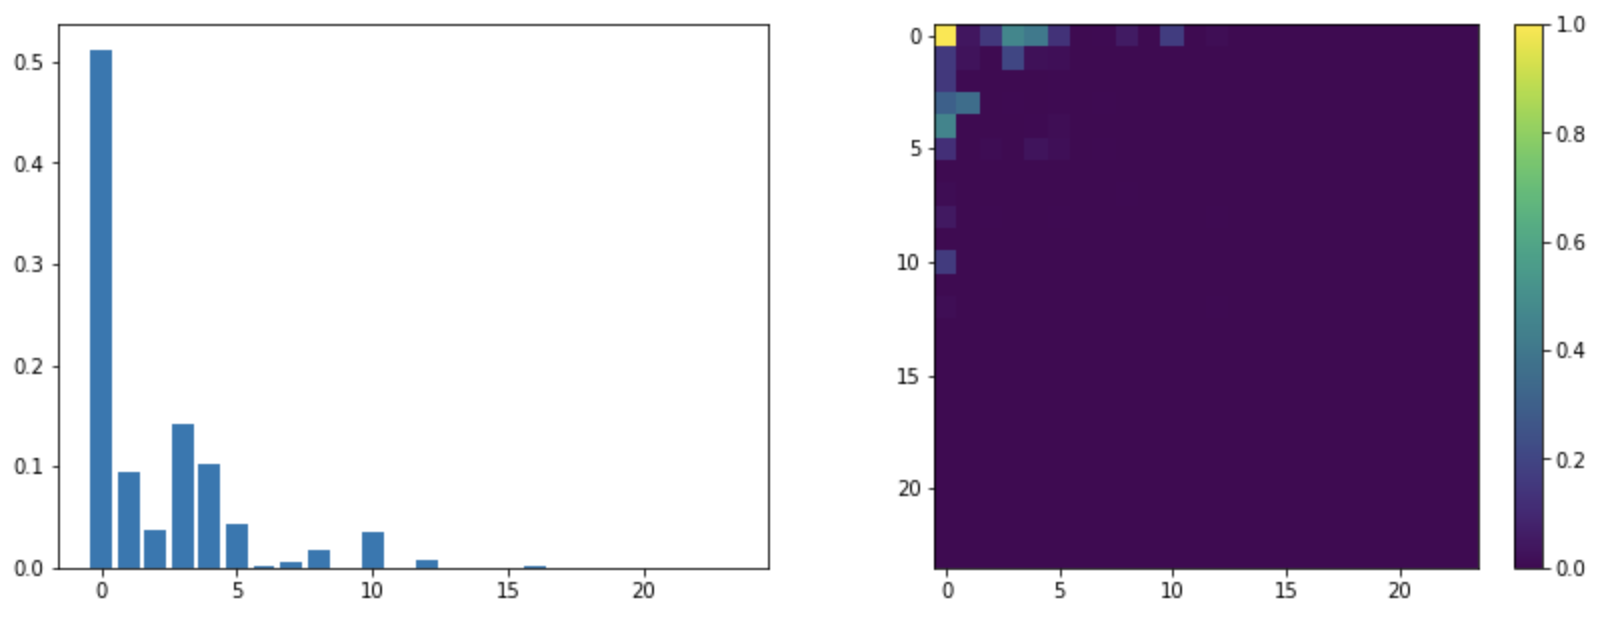
\includegraphics[scale=0.5]{rythm_hist_transition_1}
            \caption{Histogram występowania poszczególnych długości dźwięków i przejść między nimi}
            \label{rythm_hist_transition_1}
        \end{figure}
    }

    \section{Wrażenia subiektywne}
    {
        Próbki wygenerowane przez model nie dały zadowalających rezultatów. Pomimo akceptowalnego poziomu 
        harmoniczności utworów, rytmiczność pozostawia wiele do życzenia. Zdecydowanie dominującą wartością 
        rytmiczną była najkrótsza możliwa wartość. Najbardziej prawdopodobnym wytłumaczeniem tego zjawiska jest 
        problem niezrównoważenia kategorii wartości rytmicznych. 

        \bigskip

        Po dogłębnej analizie stwierdzono, że zdecydowana większość dźwięków o najkrótszym czasie trwania
        wynika z przesunięć wiadomości w plikach midi o 1 lub 2 wartości taktujące. Dla kontekstu, najczęściej stosowaną
        prędkością taktowania jest 120 taktów na ćwierćnutę. Źródłem tego zjawiska mógł być zamierzony 
        zabieg wprowadzający element niedoskonałości, mający na celu wprowadzenie ludzkiego charakteru nagrania 
        wykonywanego przez prawdziwych artystów.
        Niestety, zabieg ten uniemożliwił generowanie subiektywnie akceptowalnych sekwencji.

        Na podstawie powyższych wniosków, podjęto ponowną próbę uczenia. Tym razem, zbiór danych został
        ograniczony o powyżej opisane dźwięki. Proces uczenia i generowania został przeprowadzony w ten sam sposób
        co poprzednio. 
        %%% ZOSTAWIĆ CZY NIE
        % Na wykresach \ref{rythm_hist_2}, \ref{rythm_transition_2}, \ref{tonal_hist_2} i \ref{tonal_transition_2} widać oczywiste zmiany w miarach związanych z rytmiką.

        % %%% tutaj wykresiki tego lepszego modelu
        % %%% ilustracja tonalnego histogramu i macierzy przejść
        % \begin{figure}
        %     \centering
        %     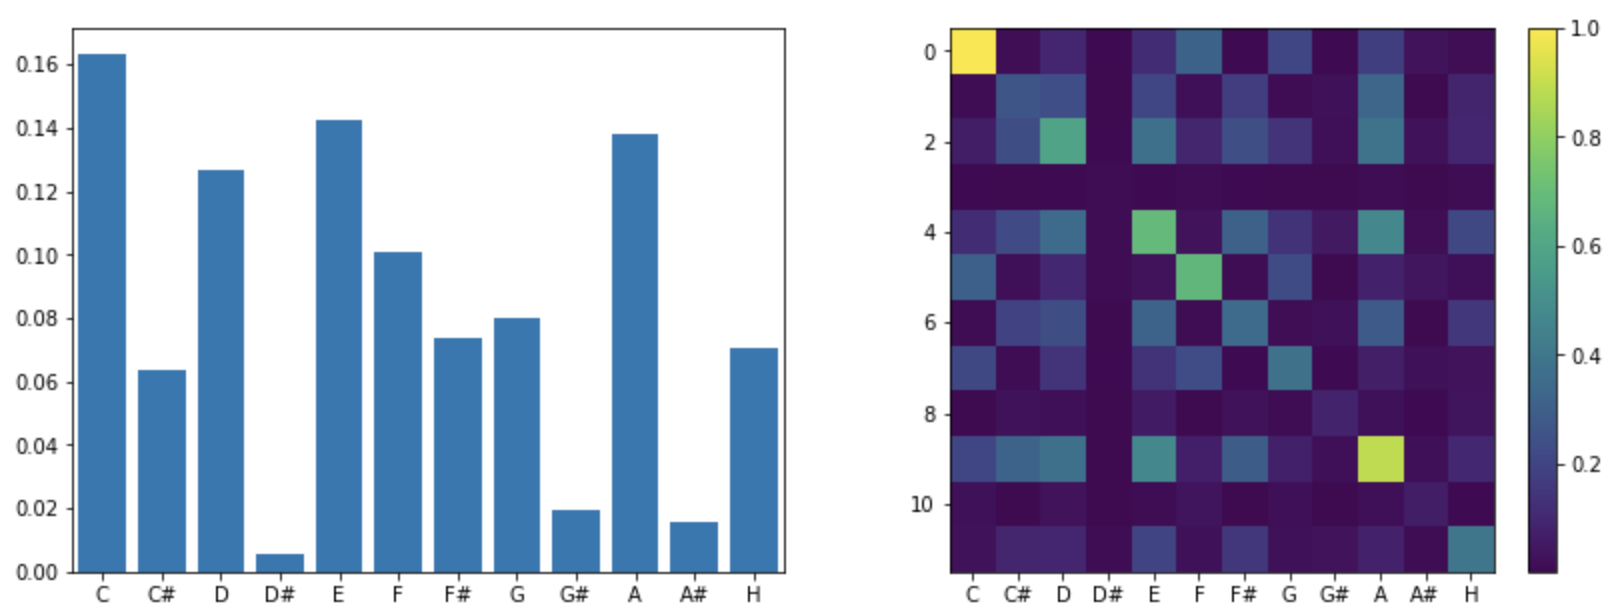
\includegraphics[scale=0.5]{tonal_hist_transition_1}
        %     \caption{Histogram występowania poszczególnych dźwięków oraz macierz przejść między nimi}
        %     \label{tonal_hist_transition_1}
        % \end{figure}

        % Jak można zaobserwować, ograniczenie zbioru danych miało również wpływ na zależności tonalne.

        %%% histogram rytmiczny i macierz przejść
        % \begin{figure}
        %     \centering
        %     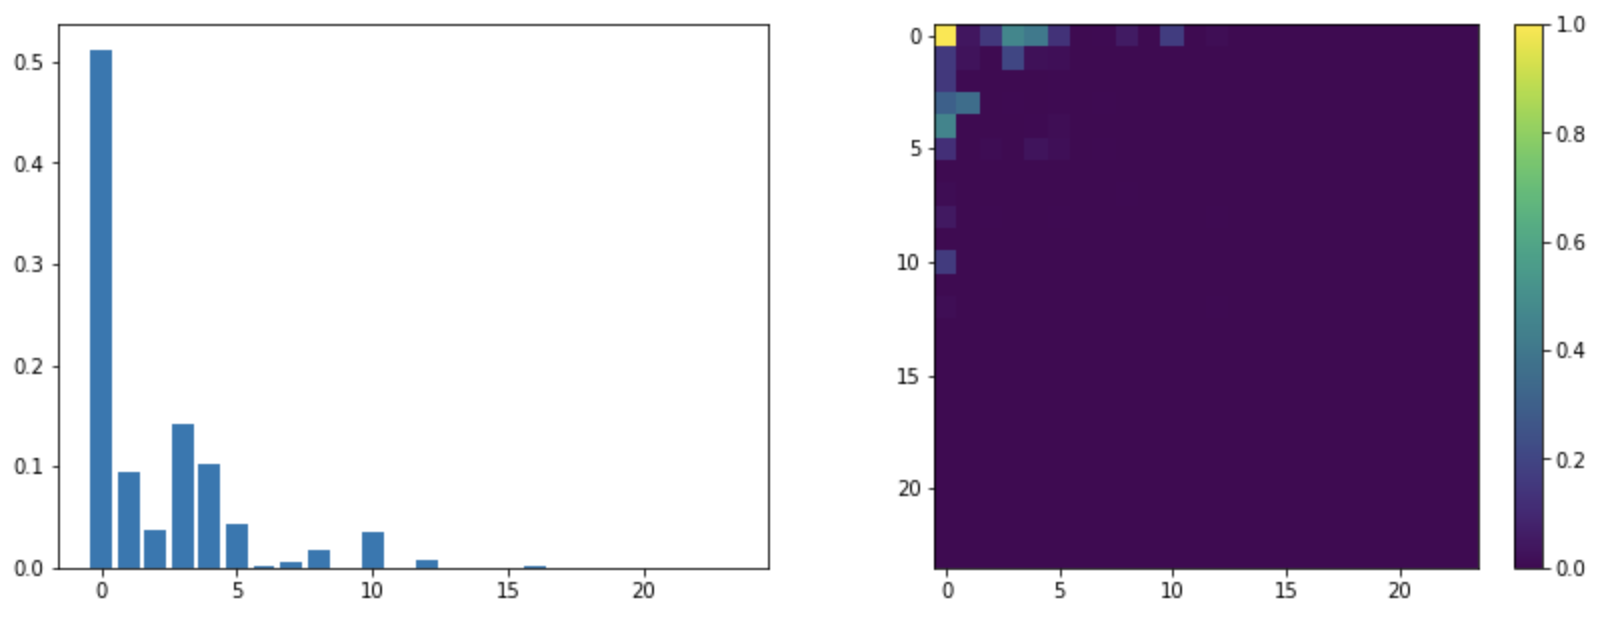
\includegraphics[scale=0.5]{rythm_hist_transition_1}
        %     \caption{Histogram występowania poszczególnych długości dźwięków i przejść między nimi}
        %     \label{rythm_hist_transition_1}
        % \end{figure}

        \bigskip

        Tym razem wyniki, choć wciąż nie idealne, były conajmniej akceptowalne. W generowanych utworach
        obserwowalny był zupełnie inny rozkład długości dźwięków. Sekwencje w subiektywnym odczuciu były dużo mniej
        chaotyczne, a zwiększone długości dźwięków pozwalały na skupienie się na następujących po sobie dźwiękach.
        
        Spośród sekwencji powstałych przy pomocy różnych ziaren, subiektywnie najbardziej interesujące wyniki
        zostały otrzymane przy początkowaniu generacji pojedynczym dźwiękiem lub pustymi wektorami.
        Fakt ten można próbować tłumaczyć pozostawieniem sieci największej swobody przy generowaniu sekwencji, lecz
        jest to jedynie spekulacja oparta na bardzo ograniczonej liczbie obserwacji.

        \bigskip

        Uzasadnione są zastrzeżenia co do tak inwazyjnej ingerencji w zbiór danych jaką jest eliminacja 
        wszystkich przedstawicieli konkretnej klasy. Z technicznego punktu widzenia bardziej poprawnym 
        rozwiązaniem mogłoby być dynamiczne skalowanie wartości błędu predykcji dla poszczególnych przypadków w czasie uczenia, 
        w taki sposób, aby mniejsza waga była przywiązywana do przedstawicieli nadreprezentowanej klasy.
    }
}